\documentclass[bigger]{beamer}

\usepackage{booktabs}
\useinnertheme{rounded}
\usecolortheme{crane}
\setbeamerfont{block title}{size={}}

\title{Exploration of the Robustness and Generalizability of the Additive Factors Model}

\author{Tom{\'a}{\v{s}} Effenberger, \textbf{Radek Pel\'anek}, Jaroslav \v{C}ech\'ak\\[10mm]
%Masaryk University Brno\\
%Czech Republic
\includegraphics[width=.3\linewidth]{al-logo}
}

\newcommand{\img}[2]{
  \begin{center}
    \includegraphics[width=#1\linewidth]{#2}
  \end{center}
}

\date{LAK 2020}

\begin{document}

\frame{\titlepage}

\begin{frame}
  \frametitle{Overview}

  \begin{itemize}
  \item AFM -- widely used student model
  \item exploration of:
    \begin{itemize}
    \item simplifying assumptions
    \item robustness, generalizability (case study)
    \end{itemize}
  \item message: more caution needed
  \end{itemize}
\end{frame}

\begin{frame}
  \frametitle{Student Modeling}

  \begin{center}
    \includegraphics[width=\linewidth]{learner-modeling-context.pdf}
  \end{center}

  \bigskip
  \begin{flushright}
    {\tiny Bayesian Knowledge Tracing, Logistic Models, and Beyond: An Overview of Learner Modeling Techniques}
  \end{flushright}
\end{frame}

\begin{frame}
  \frametitle{Additive Factors Model}

  \begin{center}
    \includegraphics[width=.4\linewidth]{afm-illustration}
  \end{center}

  \begin{itemize}
  \item family of ``logistic models''
  \item multiple skills, Q-matrix
  \item used in many studies in last 10 years -- see paper for overview
  \end{itemize}
\end{frame}

\begin{frame}
  \frametitle{Q-matrix}

  \begin{center}
      \begin{tabular}{lcccc}
    \toprule
    & $-$ & $+$ & $\times$ & () \\
    \midrule
    $10+3\times 2$ & 0 & 1 &  1 & 0 \\
    $(7-4)\times 3$ & 1 & 0 & 1 & 1 \\
    $2+ (3 + 5)$ & 0 & 1 & 0 & 1 \\
    $8-(6+2)$ & 1 & 1 & 0 & 1 \\
    $5-2\times 6$ & 1 & 0 &  1 & 0 \\
    \bottomrule
  \end{tabular}
  \end{center}
\end{frame}


\begin{frame}
  \frametitle{Additive Factors Model}

  \[ P(Y_{ij}|\alpha, \beta, \gamma) = \sigma\left(\alpha_i + \sum_{k=1}^K
    \beta_k q_{jk} + \sum_{k=1}^K \gamma_k q_{jk} t_{ik}\right) \]

\begin{itemize}
\item $i$ is student index, $j$ is item index,
\item $Y_{ij}$ is the binary response of a student $i$ on a item $j$,
\item $\sigma(x) = 1 / (1 + e^{-x})$ is the standard logistic function,
\item $K$ is the number of skills, $J$ is the number of items,
\item $Q$ is the $J\times K$ binary matrix -- $q_{jk}$ is the indicator that
  item $j$ uses skill $k$,
\item $\alpha_i$ is the proficiency (prior skill) of a student $i$,
\item $\beta_k$ is the easiness of skill $k$,
\item $\gamma_k$ is the learning rate for skill $k$,
\item $t_{ik}$ is the number of times student $i$ has practiced skill $k$
  (opportunity count).
\end{itemize}
\end{frame}

\begin{frame}
  \frametitle{Additive Factors Model}

  \begin{center}
    \includegraphics[width=.8\linewidth]{afm-illustration}
  \end{center}
\end{frame}

\begin{frame}
  \frametitle{AFM: Simplifying Assumptions}

  \begin{itemize}
  \item learning is linear (on the logit scale)
  \item effect of practice not related to observed performance
  \item observed outcomes are binary (ignoring response time, common wrong
    answers)
  \item Q-matrix is binary
  \item compensatory model of skills
  \item ignores difficulty of items
  \item ignores biases in data (e.g., items solved in fixed order)
  \end{itemize}
\end{frame}

\begin{frame}
  \frametitle{Learning Curves}

  \begin{center}
    \includegraphics[width=.8\linewidth]{learn-curve-simple}
  \end{center}
\end{frame}

\begin{frame}
  \frametitle{Types of Learning Curves}

  \begin{center}
  \begin{tabular}{llll}
    \toprule
    Type & Attempt & Opportunity & Success\\
    \midrule
    {\it empirical} & observed  & observed  & observed\\
    {\it marginal}  & observed  & observed  & predicted\\
    {\it completed} & observed  & simulated & predicted\\
    {\it idealized} & simulated & simulated & predicted\\
    \bottomrule
  \end{tabular}    
  \end{center}
\end{frame}

\begin{frame}
  \frametitle{Simulation}

  \begin{itemize}
  \item 2 skills
    \begin{itemize}
    \item skill 1: easy
    \item skill 2: difficult
    \end{itemize}
  \item 15 items 
  \item items 1-5: skill 1
  \item items 5-15: skill 1 \& 2
  \item ordering: random, fixed+skip 
  \end{itemize}
\end{frame}

\begin{frame}
  \frametitle{Learning Curves}

  \includegraphics[width=\linewidth]{learning-curves-simulated-true-model}

\end{frame}

\begin{frame}
  \frametitle{Typical AFM Application}

  \begin{itemize}
  \item take the data
  \item fit AFM model with various Q-matricies
  \item take the Q-matrix with best fit
  \item analyze (one type of) learning curves
  \end{itemize}
\end{frame}

\begin{frame}
  \frametitle{Case Study: Programming}

  \begin{columns}
    \begin{column}{0.5\linewidth}
  \begin{itemize}
  \item block-based programming
  \item 85000 attempts
  \item 5800 students
  \item 85 items
  \end{itemize}      
    \end{column}
    \begin{column}{0.5\linewidth}
  \begin{center}
    \includegraphics[width=\linewidth]{robomise}
  \end{center}      
    \end{column}
  \end{columns}

  \bigskip
  open source, data available:\\
  \url{en.robomise.cz} \\
  T. Effenberger. Blockly Programming Dataset. CSEDM 2019
\end{frame}

\begin{frame}
  \frametitle{Questions: Generalizability and Robustness}

  \begin{itemize}
  \item Does the model (AFM) fit well data in this domain?
  \item Can we use the model to select good Q-matrix?
  \item Do the learning curves provide useful insight?
  \item How robust are the result with respect to methodological choices?
  \end{itemize}
\end{frame}

\begin{frame}
  \frametitle{Q-matricies}

  \begin{center}
  \begin{tabular}{p{0.08\linewidth}p{0.82\linewidth}}
    \toprule
    Name & Skills\\
    \midrule
    Q1 & \emph{teleports}, \emph{collectables}, \emph{obstacles},
    \emph{destructibles}, \emph{program length limit}, sequences, while,
    repeat, loop, nested-loops, if, else, test, nested control structures,
    comparison\\
    Q2 & \emph{teleports}, \emph{collectables}, \emph{obstacles},
    \emph{destructibles}, sequences, while, repeat, nested loops, if, else\\
    Q3 & sequences, while, repeat, nested loops, if, else\\
    Q4 & sequences, loop, nested loops, test\\
    \bottomrule
  \end{tabular}    
  \end{center}
\end{frame}

\begin{frame}
  \frametitle{Models}

  \begin{itemize}
  \item baselines: global average, item average
  \item AFM-BG: AFM without $\alpha$ parameter (student skill)
  \item AFM-ABG: full AFM 
  \item AFM-BGT: AFM-BG model with item difficulties
  \end{itemize}
\end{frame}

\begin{frame}
  \frametitle{Results: Effect of Data Filtering}

  \begin{center}
    \includegraphics[width=\linewidth]{student-filtering-effect}
  \end{center}
\end{frame}

\begin{frame}
  \frametitle{Results: Cross-validation Setting}

  \begin{center}
    \includegraphics[width=\linewidth]{cv-effect}
  \end{center}
\end{frame}

\begin{frame}
  \frametitle{Results: Model Comparison}

  \begin{center}
    \includegraphics[width=.5\linewidth]{programming-metrics}
  \end{center}
\end{frame}

\begin{frame}
  \frametitle{Results: Learning Curves}

  \begin{center}
    \includegraphics[width=.6\linewidth]{learning_curves}
  \end{center}
\end{frame}

\begin{frame}
  \frametitle{Conclusions}

  \begin{itemize}
  \item studies using AFM: more caution necessary
  \item AFM has many simplifying assumptions, not satisfied in practice
  \item out-of-the-box application $\Rightarrow$ possibly misleading
    conclusions
  \item basic precaution: comparison with ``item average'' predictor
  \end{itemize}

\end{frame}

\begin{frame}
  \frametitle{Questions}

  \begin{center}
    \includegraphics[width=.5\linewidth]{al-logo}
  \end{center}

  Contact:\\
  Radek Pel\'anek\\
  \texttt{xpelanek@fi.muni.cz}\\
  \texttt{https://www.fi.muni.cz/adaptivelearning/}
\end{frame}


\end{document}